% 03_hw

\subsection{Quantenmechanische Betrachtung}

\begin{frame}
  \frametitle{Repetition Wasserstoffatom}
	\begin{columns}
		 \column{.5\textwidth}
			 \begin{itemize} 
			\item[]	$h\nu = \Delta E$ 
			\item[]   $h:$ Planksches  Wirkungsquantum
		 	\item[]   $\nu:$ Frequenz
		 	\item[]   $E: $ Energie
		 	\end{itemize}
		 	\vspace{.5cm}		 	 
		 	�bergang $\infty \rightarrow 1: \lambda_1 = 91nm$
		 	
		 	$\nu_1 = \dfrac{c}{\lambda_1} = 3.3 PHz \quad(10^{15})$
		 	\vspace{.5cm}
		 	
		 	�bergang $6 \rightarrow 5: \lambda_2 = 7457nm$
		 	
		 	$\nu_2 = \dfrac{c}{\lambda_2} = 40,2 THz$
		 			 	
		\column{.5\textwidth}
		 	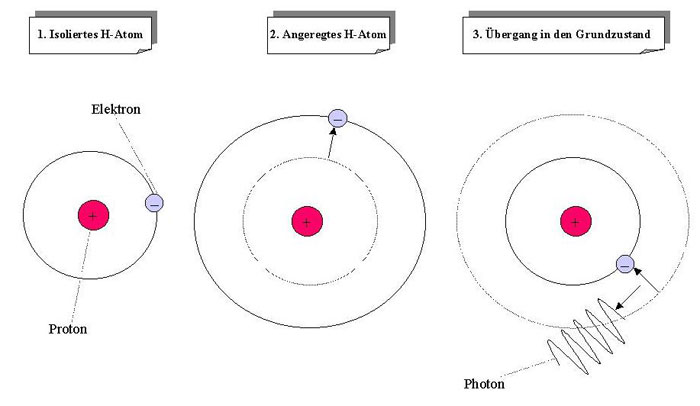
\includegraphics[width = 5cm]{./pictures/wasserstoffBohr}
		 	
		 	Spektrum Balmer-Serie
		 	
		 	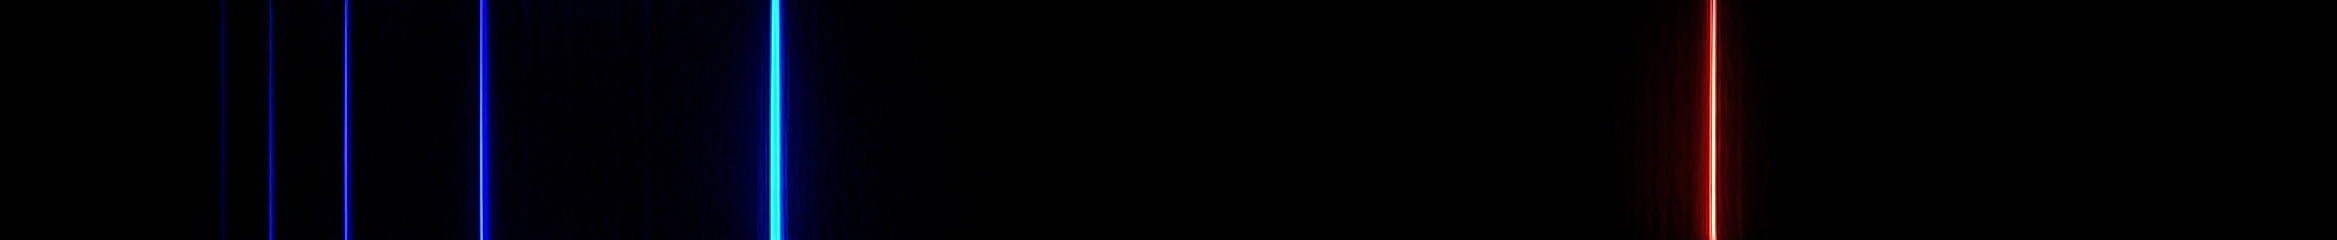
\includegraphics[width = 5cm]{./pictures/wasserstoffSpektrum}
	
	\end{columns}

\end{frame}

\begin{frame}
  \frametitle{Feinstruktur�bergang}
	\begin{columns}
		\column{.5\textwidth}
		\begin{itemize}
		\item[] Betrachtung Spektrum
		\item[] Spin-Bahn Kopplung
		\end{itemize}
		
		\column{.5\textwidth}
		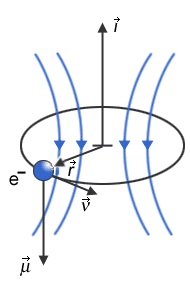
\includegraphics[width = 4cm]{./pictures/feinstrukturelektron}
		
	
		
	\end{columns}
	
\end{frame}

\begin{frame}
	\frametitle{Hyperfeinstruktur�bergang}
	Wechselwirkung zwischen Spin und elektron
	Anwendung St�rungstheorie -> kleine Effekte summieren sich
	Atom haben niedriges niveau -> anregung -> einige werden h�heres Niveau bekommen
	
\end{frame}

\begin{frame}
	\frametitle{Alkalimetalle}
	Abgeschlossene Schalen haben verschwindenden Drehimplus -> nur �usserstes elektron reagiert
	1 Valenzelektron
\end{frame}


%%% Local Variables: 
%%% mode: latex
%%% TeX-master: "../main"
%%% End: 
